\subsection{Experiments with Real-world Application}
\label{exp:idol2}

We performed a second series of experiments, namely place recognition
in an indoor environment, to evaluate our algorithm. We considered a
realistic scenario where the algorithm had to incrementally update the
model, so to adapt to the variations in an indoor environment due to
human activities over long time spans. These variations include people
appearing in different rooms during working time, objects such as cups
moved or taken in/out of the drawers, pieces of furniture pushed
around, and so forth.

\begin{figure*}[t]
\centering \footnotesize
\begin{tabular}{@{}c@{\hspace{0.002\linewidth}}c@{\hspace{0.002\linewidth}}
c@{\hspace{0.002\linewidth}}c@{\hspace{0.002\linewidth}}
c@{\hspace{0.002\linewidth}}c@{\hspace{0.002\linewidth}}
c@{\hspace{0.002\linewidth}}c@{}}
% -------------------------------------------------------------------
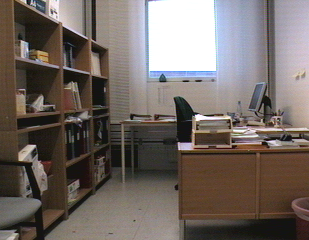
\includegraphics[width=0.123\linewidth]{figs/idol/bo_cloudy.png} &
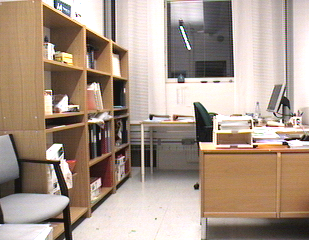
\includegraphics[width=0.123\linewidth]{figs/idol/bo_night.png}  &
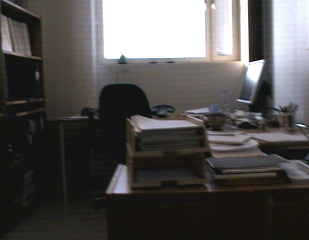
\includegraphics[width=0.123\linewidth]{figs/idol/bo_sunny.png}  &
\includegraphics[width=0.123\linewidth]{figs/idol/cr_cloudy.png} &
\includegraphics[width=0.123\linewidth]{figs/idol/cr_night.png}  &
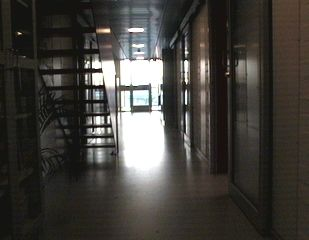
\includegraphics[width=0.123\linewidth]{figs/idol/cr_sunny.png} &
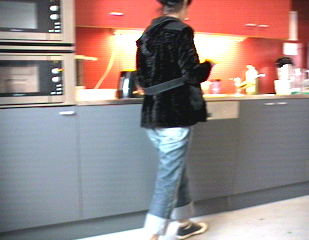
\includegraphics[width=0.123\linewidth]{figs/idol/people1.png}  &
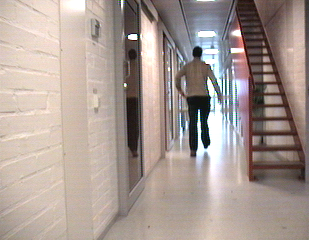
\includegraphics[width=0.123\linewidth]{figs/idol/people2.png}  \\
% -------------------------------------------------------------------
\includegraphics[width=0.123\linewidth]{figs/idol/cup1.png}   &
\includegraphics[width=0.123\linewidth]{figs/idol/cup3.png}   &
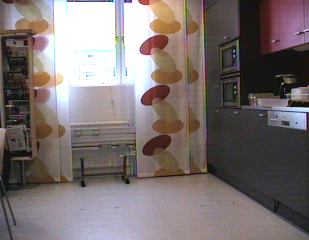
\includegraphics[width=0.123\linewidth]{figs/idol/chair1.png}   &
\includegraphics[width=0.123\linewidth]{figs/idol/chair3.png} &
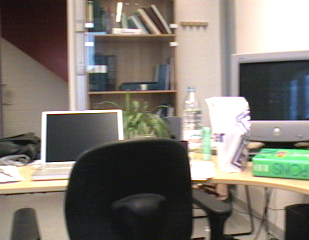
\includegraphics[width=0.123\linewidth]{figs/idol/time1.png} &
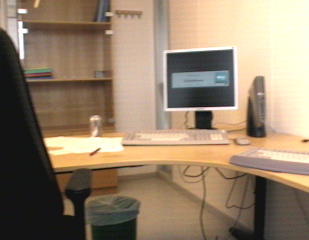
\includegraphics[width=0.123\linewidth]{figs/idol/time2.png} &
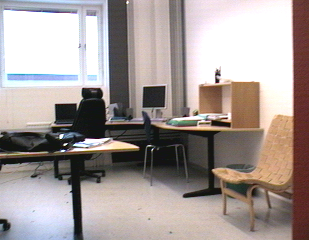
\includegraphics[width=0.123\linewidth]{figs/idol/time3.png}  &
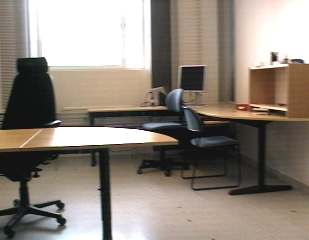
\includegraphics[width=0.123\linewidth]{figs/idol/time4.png}  \\
% -------------------------------------------------------------------
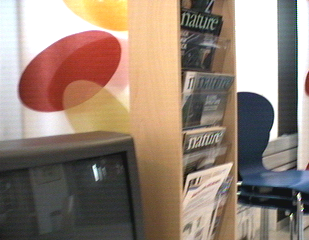
\includegraphics[width=0.123\linewidth]{figs/idol/drive1.png}   &
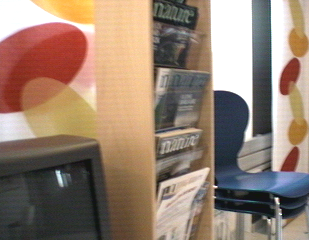
\includegraphics[width=0.123\linewidth]{figs/idol/drive2.png}   &
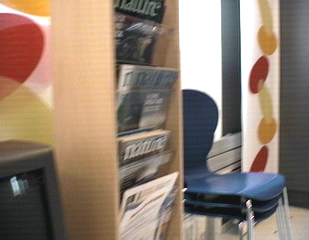
\includegraphics[width=0.123\linewidth]{figs/idol/drive3.png}   &
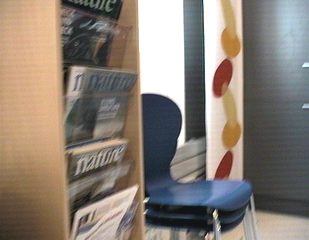
\includegraphics[width=0.123\linewidth]{figs/idol/drive4.png} &
\includegraphics[width=0.123\linewidth]{figs/idol/drive5.png} &
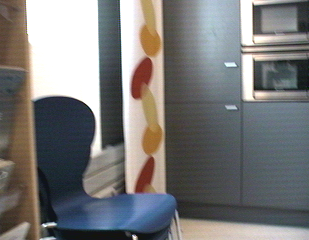
\includegraphics[width=0.123\linewidth]{figs/idol/drive6.png} &
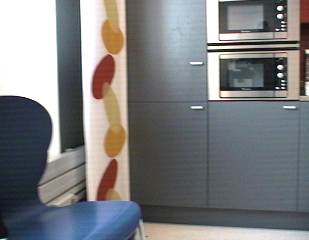
\includegraphics[width=0.123\linewidth]{figs/idol/drive7.png}  &
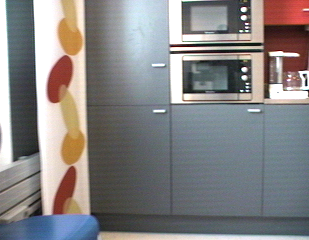
\includegraphics[width=0.123\linewidth]{figs/idol/drive8.png}   \\
% -------------------------------------------------------------------
\end{tabular}
\caption{Sample images illustrating the variations captured in the IDOL2 database.
Images in the top row show the variability introduced by changes in
illumination for two rooms (first six images) as well as people
appearing in the environment.  The middle row shows the influence of
people's everyday activity (first four images) as well as larger
variations which happened over a time span of $6$ months. Finally, the
bottom row illustrates the changes in viewpoint observed for a series
of images acquired one after another in $1.6$ seconds.}
\label{fig:idol}
\end{figure*}

Experiments were conducted on a newly introduced database called IDOL2
(Image Database for rObot Localization 2, \cite{luo:idol2}), which
contains $24$ image sequences acquired using a perspective camera
mounted on two mobile robot platforms. The acquisition was performed
within an indoor laboratory environment consisting of five rooms of
different functionality. The sequences were acquired under various
weather and illumination conditions (sunny, cloudy, and night) and
across a time span of six months. Thus, this data capture natural
variability that occurs in real-world environments because of both
natural changes in the illumination and human
activity. Fig. \ref{fig:idol} shows some sample images from the
database, illustrating the difficulties of the task.  The image
sequences in the database are divided as follows: for each robot
platform and for each type of illumination conditions, there were four
sequences recorded. Of these four sequences, the first two were
acquired six months before the last two. This means that, for each
robot and for every illumination condition, there are always two
sequences acquired under similar conditions, and two sequences
acquired under very different conditions. This makes the database
suitable for different kinds of evaluation on the adaptability of an
incremental algorithm. For further details about the database, we
refer the readers to \cite{luo:idol2}.

The evaluation was performed using composed receptive field histograms
(CRFH) \cite{linde:icpr04} as global image features and SIFT
\cite{lowe99object} for extracting local features. In the experiments,
we consider both exponential $\chi^2$ kernel for SVM (when use CRFH),
and local kernels \cite{wallraven:iccv03} (SIFT).  Similarly to the
previous set of experiments, we run the OISVM using different values
of $\eta$, for both kernels.

We benchmarked OISVM against two approximate incremental SVM
extensions: the standard fixed-partition technique
\cite{syed99incremental} and the memory-controlled incremental SVM
\cite{pronobis:icvs06}, a recently introduced version of incremental SVM,
inspired by the work of Downs et~al. \cite{DownsGM01}; this replicates
the experimental setup of \cite{luo:icra07}, thus allowing for a
straightforward comparison between exact and approximate methods on
this task
\footnote{We gratefully thank Jie Luo who gave us the software and assistance 
nnecessary to replicate the experiments.}.  
The algorithm was trained incrementally on three sequences
from IDOL2, acquired under similar illumination conditions with the
same robot platform; the fourth sequence was used for testing. In
order to test the various properties of interest of the incremental
algorithms, we need a reasonable number of incremental steps.  Thus,
every sequence was splitted into $5$ subsequences, so that each subset
contained one of the five images acquired by the robot every second
(image sequences were acquired at a rate of 5fps). Since during
acquisition the camera's viewpoint continuously changes
\cite{luo:icra07}, the subsequences could be considered as recorded
separately in a static environment but for varying pose.  This setup
allows us to examine how the algorithms perform on data with less
variations. In order to get a feeling of the variations of the frame
images in a sequence, bottom row of Fig. \ref{fig:idol} shows some
sample images acquired within a time span of 1.6 sec. This setup
allows us to examine how the algorithms perform on data with less
variations. As a result, training on each sequence was performed in 5
steps, using one subsequence at a time, resulting in 15 steps in
total. Overall, we considered 36 different permutations of training
and test sequences for the exponential $\chi^2$ kernel and 12
permutations for the matching kernel \footnote{Upon acceptance of the
paper, we will report results on 36 permutations for the matching
kernel as well (experiments currently running).}; here we report
average results with standard deviation. Fig. \ref{fig:exp:idol},
left, shows the recognition rates of the exponential $\chi^2$ kernel
(top) and matching kernel (bottom) experiments obtained at each step
using OISVM and the other approximate incremental
algorithms. Fig. \ref{fig:exp:idol}, right, reports the number of
support vectors stored in the model at each step of the incremental
procedure, for both kernel types.

We see that, performance-wise, all methods achieves statistically
comparable results; this is true for both kernel types. Regarding the
growth of the SV solution as the incremental steps grow, the OISVM
algorithm shows a considerable advantage with respect to the fixed
partition and the memory controlled incremental methods. In the case
of the exponential $\chi^{2}$ kernel this advantage is truly
impressive (Fig \ref{fig:exp:idol}, top right): for $\eta=0.017$ and
$0.025$ the reduction in the number of stored SV is of $34\%/21\%$
(final incremental step) and compared to the fixed-partition method,
and of $55\%/36\%$ (final incremental step) with respect to the
memory-controlled algorithm. Even more important, OISVM, for these two
values of $\eta$, has found a plateau in memory, while for the other
two methods the trend seems to be of a growth (less pronounced for the
memory controlled algorithm, which plot might be interpreted as an
asymptotic plateau) proportional to the number of training data. Note
that the choice of the parameter $\eta$ is crucial for achieving an
optimal trade-off between compactness of the solution and optimal
performance.

It is very interesting to note that, in the case of the matching
kernel, the memory reduction for OISVM is less pronounced with respect
to the memory-controlled method, and there isn't a clear plateau in
memory growth by any of the algorithms.  This behavior might be due to
several factors: to begin with, the matching kernel is not a Mercer
kernel \cite{fleuret:bmvc04}, which might affect the algorithm. Also,
the algorithm might not reach a plateau in the SVs growth because, in
the induced space of the matching kernel, there seems to be a high
probability that couples training points are orthogonal or almost
orthogonal (note that as the kernel is not a Mercer one, the geometric
interpretation might not be valid).

We can conclude that these results are in agreement with those
obtained on the machine learning benchmark databases, and show the
effectiveness of OISVM in controlling the growth of the SV solution
for online learning scenarios.

\begin{figure*}[t]
  \centering \footnotesize
  \begin{tabular}{c@{\hspace{0.5cm}}c}
  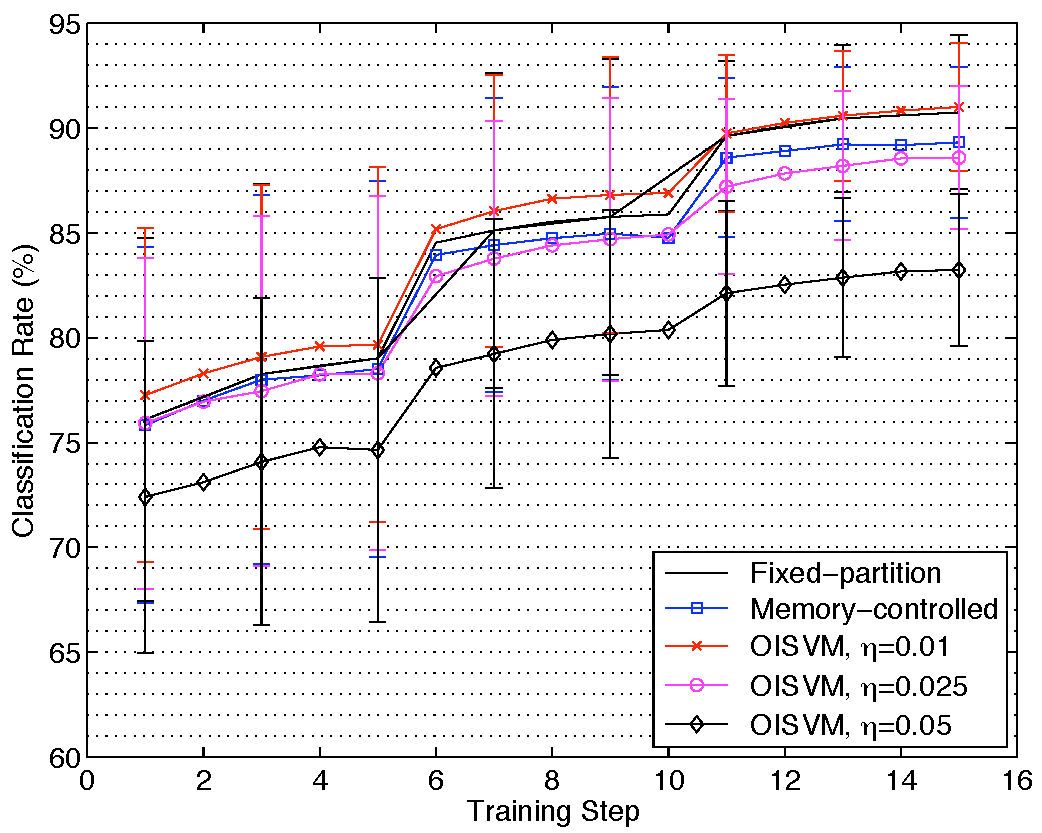
\includegraphics[width=0.47\linewidth]{figs/results/chi_cr} &
  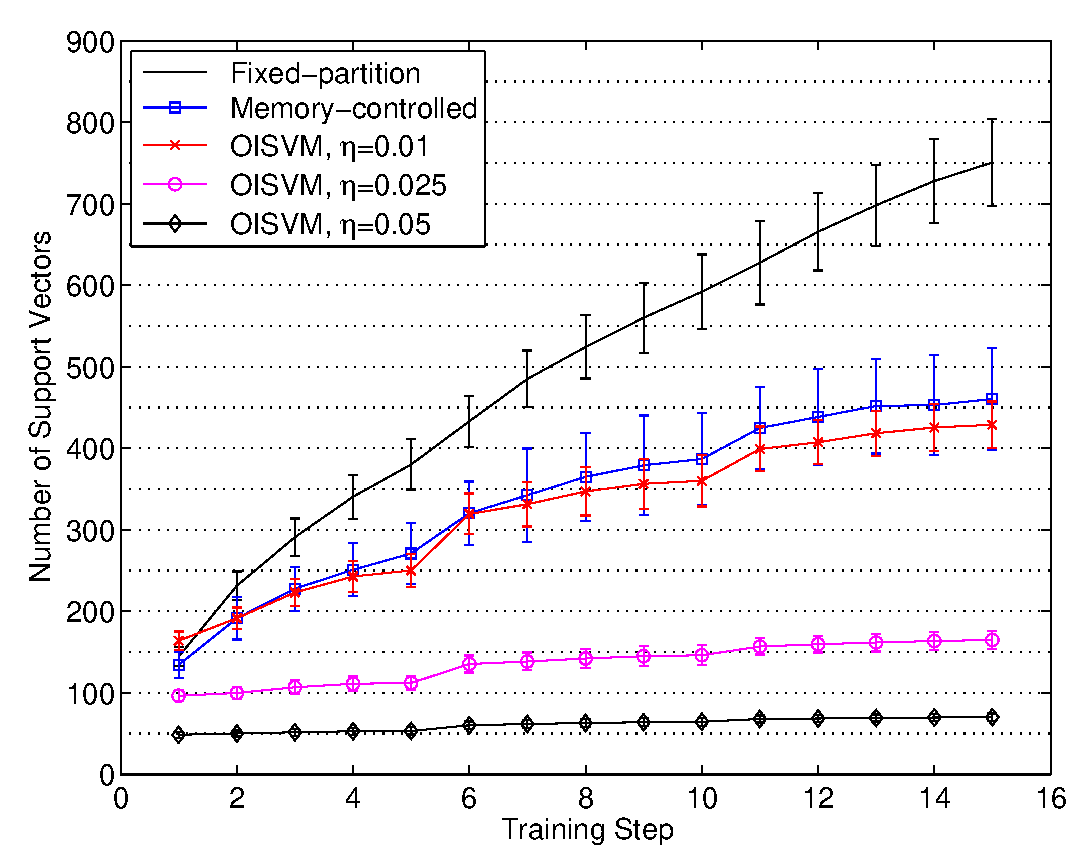
\includegraphics[width=0.47\linewidth]{figs/results/chi_sv} \vspace{0.1cm}\\
  \multicolumn{2}{c}{(a)~Number of support vectors and classification rate obtained at each incremental step using $\chi^2$ kernel.}  \\
  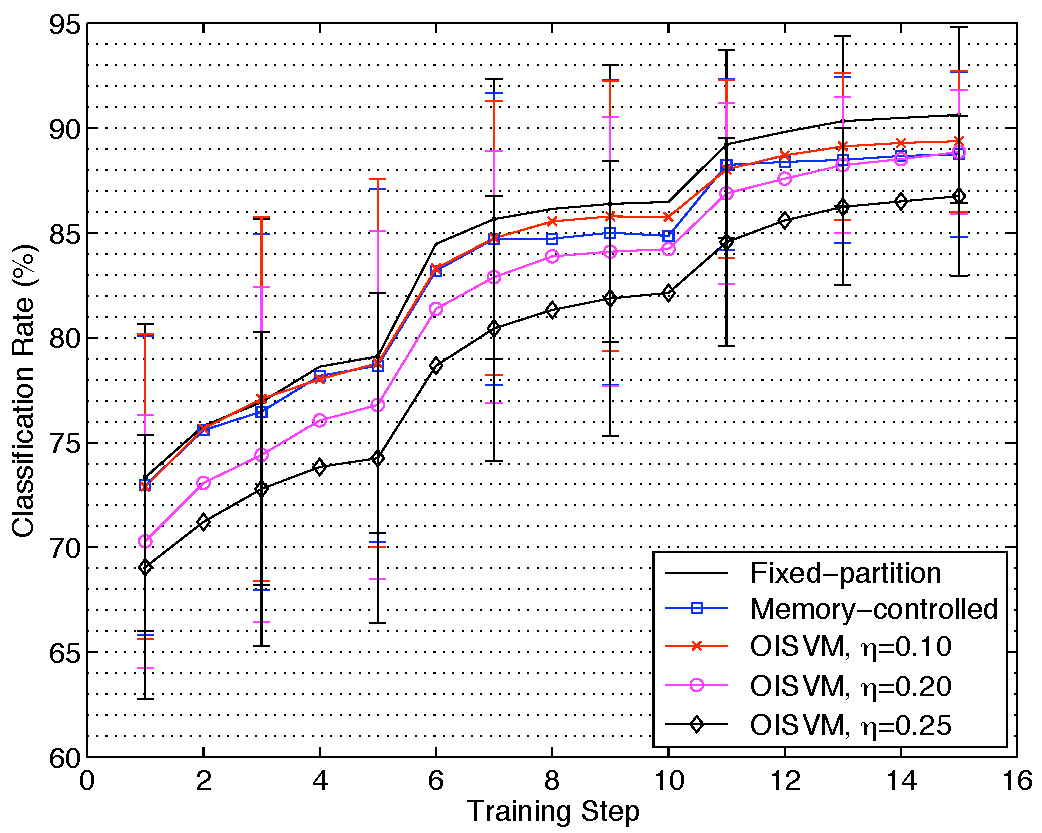
\includegraphics[width=0.47\linewidth]{figs/results/local_cr} &
  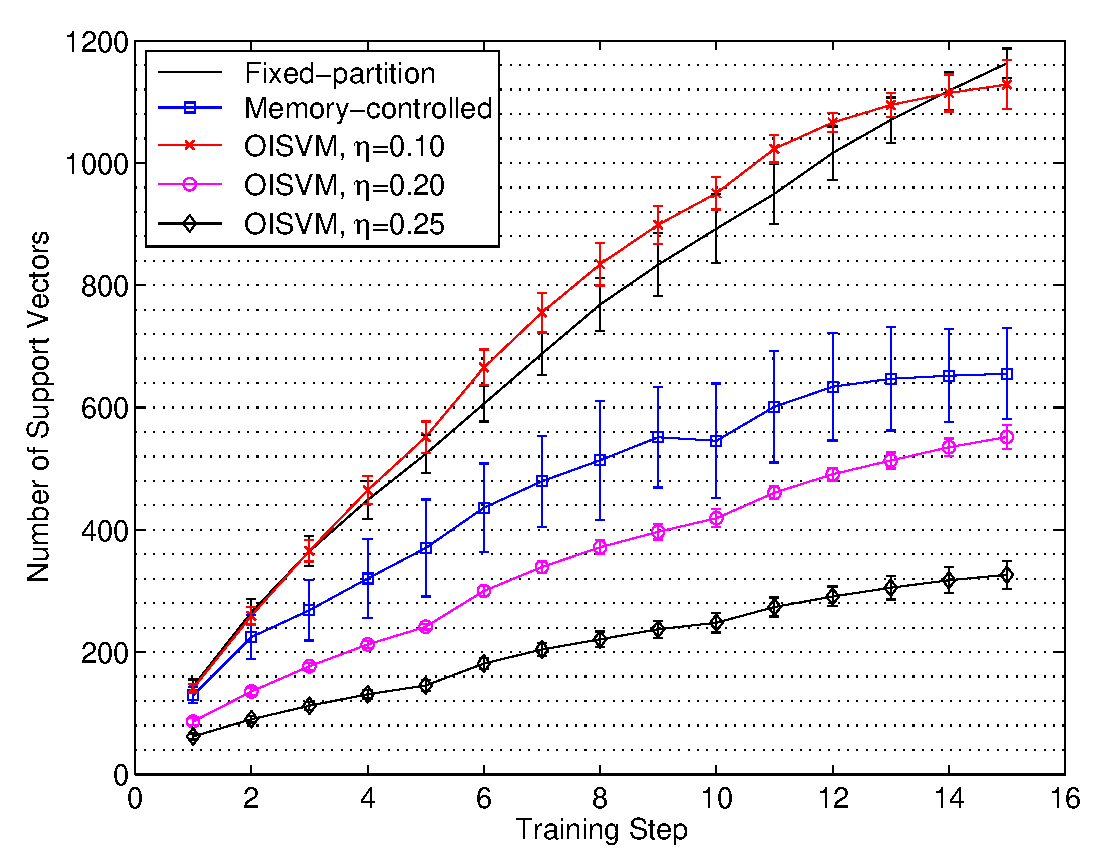
\includegraphics[width=0.47\linewidth]{figs/results/local_sv} \vspace{0.1cm}\\
  \multicolumn{2}{c}{(b)~Number of support vectors and classification rate obtained at each incremental step using local kernel.} \\
  \end{tabular}
\caption{Average results obtained for experiment performed on the IDOL2 database, using
         OISVM with  three different values of $\eta$, the 
         fixed-partition and memory-controlled methods. }
\label{fig:exp:idol}
\end{figure*}
